% Unofficial Purdue University Poster Template
% based on
% https://github.com/k4rtik/uchicago-poster
% a fork of https://github.com/anishathalye/gemini

\documentclass[final]{beamer}

% ====================
% Packages
% ====================

\usepackage[T1]{fontenc}
\usepackage{lmodern}
\usepackage[size=custom,width=120,height=72,scale=1.0]{beamerposter}
% Self-contained Purdue-inspired theme; no external Gemini files required.
\definecolor{PurdueGold}{HTML}{CFB991}
\definecolor{PurdueBlack}{HTML}{000000}
\definecolor{PurdueLight}{HTML}{F5F1E9}
\definecolor{Ocean}{HTML}{176B87}
\definecolor{OceanLight}{HTML}{E7F3F7}
\definecolor{Plum}{HTML}{724B83}
\definecolor{PlumLight}{HTML}{F1EAF5}
\definecolor{Leaf}{HTML}{357052}
\definecolor{LeafLight}{HTML}{EAF4EE}
\definecolor{Rust}{HTML}{AC4934}
\setbeamercolor{normal text}{fg=PurdueBlack,bg=white}
\setbeamercolor{headline}{fg=white,bg=PurdueBlack}
\setbeamercolor{footline}{fg=PurdueBlack,bg=PurdueGold}
\setbeamercolor{block title}{fg=PurdueBlack,bg=white}
\setbeamercolor{block body}{fg=PurdueBlack,bg=white}
\setbeamercolor{block title alerted}{fg=PurdueBlack,bg=PurdueGold}
\setbeamercolor{block body alerted}{fg=PurdueBlack,bg=PurdueLight}
\setbeamercolor{block title example}{fg=PurdueBlack,bg=PurdueGold}
\setbeamercolor{block body example}{fg=PurdueBlack,bg=PurdueLight}
\setbeamercolor{itemize item}{fg=PurdueBlack}
\setbeamercolor{itemize subitem}{fg=PurdueBlack}
\setbeamercolor{enumerate item}{fg=PurdueBlack}
\setbeamerfont{title}{size=\fontsize{64}{72}\selectfont,series=\bfseries}
\setbeamerfont{author}{size=\fontsize{32}{40}\selectfont}
\setbeamerfont{institute}{size=\fontsize{28}{36}\selectfont}
\setbeamerfont{block title}{size=\fontsize{34}{40}\selectfont,series=\bfseries}
\setbeamerfont{block title alerted}{parent=block title}
\setbeamerfont{block title example}{parent=block title}
\setbeamertemplate{navigation symbols}{}
\setbeamertemplate{caption}[numbered]
\setbeamertemplate{blocks}[default]
\newcommand{\heading}[1]{\par\medskip{\bfseries #1}\par\smallskip}
\newcommand{\footercontent}[1]{\def\posterfooter{#1}}
\setbeamertemplate{headline}{%
  \begin{beamercolorbox}[wd=\paperwidth,sep=1.5cm,center]{headline}
    {
\includegraphics[width=23cm]{images/purdue-logo.png}\par}
    \vskip0.6cm
    {\usebeamerfont{title}\inserttitle\par}
    \vskip0.6cm
    {\usebeamerfont{author}\insertauthor\par}
    \vskip0.4cm
    {\usebeamerfont{institute}\insertinstitute\par}
  \end{beamercolorbox}
  {\color{PurdueGold}\rule{\paperwidth}{0.35cm}}
  \vskip0.8cm
}
\setbeamertemplate{footline}{%
  \begin{beamercolorbox}[wd=\paperwidth,sep=0.7cm]{footline}
    \fontsize{22}{28}\selectfont\posterfooter
  \end{beamercolorbox}
}
\usepackage{graphicx}
\usepackage{booktabs}
\usepackage{doi}
\usepackage[numbers]{natbib}
\usepackage[patch=none]{microtype}
\usepackage{tikz}
\usetikzlibrary{positioning,arrows.meta,shapes.geometric}
\usepackage{pgfplots}
\pgfplotsset{compat=1.18}
\usepackage{anyfontsize}

\pdfstringdefDisableCommands{%
\def\translate#1{#1}%
}

% ====================
% Lengths
% ====================

% If you have N columns, choose \sepwidth and \colwidth such that
% (N+1)*\sepwidth + N*\colwidth = \paperwidth
\newlength{\sepwidth}
\newlength{\colwidth}
\setlength{\sepwidth}{0.025\paperwidth}
\setlength{\colwidth}{0.3\paperwidth}

\newcommand{\separatorcolumn}{\begin{column}{\sepwidth}\end{column}}


% Draft based on user-provided project abstract and repository code at
% 87a5b301c5aca2775e9d210042a21a07fc038493 (2026-11-02).
% Current four-PDF smoke check: poster/evidence/paper-check-2026-11-12.json.
% Candidate counts measure execution coverage, not extraction correctness.
% Authors supplied by the user in the Team 2 membership screenshot.
% Title follows the user-confirmed onboarding framing.
% TODO: Confirm venue, demonstration PDF and metric names.
% Cross-team roles: user-shared Landseer Agent Tools.xlsx, team 1--4 sheets.
\title{Agentic Onboarding Tools for Empirical\\Evaluation of Machine Learning Defenses}
\author{Aarush Kumar \and Andrew Zeng \and Benjamin Taylor \and Bhanu Adaveni \and Rudra Vaishnav \and Yuchao Shen}
\institute{Purdue University}
\footercontent{\href{https://github.com/Auspr7ng/fair_fairness_benchmark}{github.com/Auspr7ng/fair\_fairness\_benchmark}\hfill Working draft \enspace | \enspace November 2026}
\setbeamercolor{caption name}{fg=PurdueBlack}
\setbeamerfont{block body}{size=\fontsize{27}{34}\selectfont}
\setbeamerfont{block body alerted}{parent=block body}
\setbeamerfont{block body example}{parent=block body}
\setlength{\parskip}{0.45em}

% Reusable original vector illustrations; no generated experimental imagery.
\tikzset{arr/.style={-{Latex[length=5mm]},line width=1.8pt},lab/.style={align=center,font=\fontsize{25}{31}\selectfont},smalllab/.style={align=center,font=\fontsize{22}{28}\selectfont}}
\newcommand{\papericon}[3]{%
  \begin{scope}[shift={(#1,#2)}]
  \draw[fill=white,draw=#3,line width=2pt] (-2,-2.6)--(2,-2.6)--(2,1.6)--(1,2.6)--(-2,2.6)--cycle;
  \draw[draw=#3,line width=1.5pt] (1,2.6)--(1,1.6)--(2,1.6);
  \foreach \y in {-1.5,-0.5,0.5,1.5}{\draw[draw=#3,line width=1.2pt] (-1.4,\y)--(0.5,\y);}
  \end{scope}}
\begin{document}
\begin{frame}[t]
\begin{columns}[t]
\separatorcolumn
\begin{column}{\colwidth}
\begin{block}{1 \enspace ML is everywhere. So are its risks.}
\begin{center}
\begin{tikzpicture}[x=1cm,y=1cm]
% Healthcare, transport and finance: pictograms rather than text panels.
\draw[fill=OceanLight,draw=Ocean,line width=2pt] (-12,-1.5) rectangle (-6,3.7);
\draw[fill=Ocean,draw=none] (-10.9,0.3) rectangle (-7.1,1.5);
\draw[fill=Ocean,draw=none] (-9.6,-1) rectangle (-8.4,2.8);
\node[smalllab] at (-9,-3) {Healthcare};
\draw[fill=PlumLight,draw=Plum,line width=2pt,rounded corners=8pt] (-3,-0.8) rectangle (3,1.8);
\draw[draw=Plum,line width=2pt] (-2,1.8)--(-1,3.4)--(1,3.4)--(2,1.8);
\foreach \x in {-1.9,1.9}{\draw[fill=Plum] (\x,-0.8) circle (0.6);}
\node[smalllab] at (0,-3) {Transportation};
\draw[fill=LeafLight,draw=Leaf,line width=2pt] (6,2.7)--(9,4.2)--(12,2.7)--cycle;
\foreach \x in {7,9,11}{\draw[draw=Leaf,line width=4pt] (\x,-0.6)--(\x,2.5);}
\draw[draw=Leaf,line width=3pt] (6,-1)--(12,-1);
\node[smalllab] at (9,-3) {Finance};
\draw[arr,draw=Rust] (-9,-4.3)--(-9,-6);
\draw[arr,draw=Rust] (0,-4.3)--(0,-6);
\draw[arr,draw=Rust] (9,-4.3)--(9,-6);
\node[lab,text=Rust] at (0,-7.4) {Manipulated inputs \quad Poisoned data\\Privacy leakage};
\end{tikzpicture}
\end{center}
\begin{itemize}
\item Attacks can cause unsafe predictions or expose sensitive data~[1].
\item Defenses address individual threats, but their \textbf{combined effects are hard to predict}.
\item We need to test defenses together, not just in isolation.
\end{itemize}
\end{block}
\vspace{0.8cm}
\begin{block}{2 \enspace Landseer: test defense combinations}
\begin{itemize}
\item A framework for integrating defenses and measuring their interactions~[1].
\item Onboard tools $\rightarrow$ explore pipelines $\rightarrow$ analyze interference.
\end{itemize}
\begin{figure}
\centering
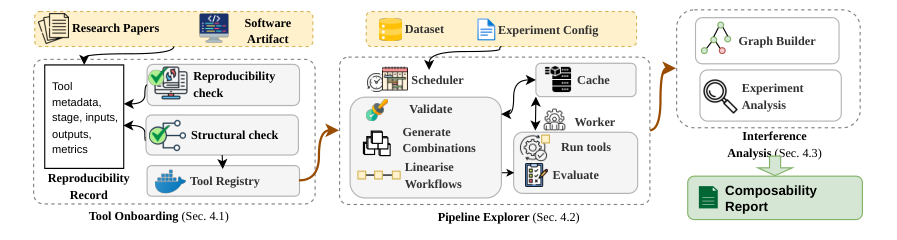
\includegraphics[width=\linewidth]{images/landseer-system.png}
\end{figure}
{\fontsize{21}{27}\selectfont Landseer system overview. Reproduced from Sharma et al., Fig. 1~[1], CC BY 4.0. The existing framework is prior work.}
\end{block}
\vspace{0.8cm}
\begin{alertblock}{The onboarding bottleneck}
\begin{itemize}
\item Research papers and code use inconsistent metrics, environments, and interfaces.
\item \textbf{Our focus:} automate paper metric extraction and reference-record preparation.
\end{itemize}
\end{alertblock}
\end{column}
\separatorcolumn
\begin{column}{\colwidth}
\begin{block}{3 \enspace Toward agentic tool onboarding}
\begin{center}
\begin{tikzpicture}[x=1cm,y=1cm]
% Research artifacts above the agent.
\papericon{-10}{0}{Ocean}
\node[lab] at (-10,-4) {Paper};
\draw[fill=PlumLight,draw=Plum,line width=2pt] (6,-2.4) rectangle (14,2.4);
\node[font=\fontsize{52}{58}\selectfont,text=Plum] at (10,0) {\texttt{</>}};
\node[lab] at (10,-4) {Code};
% Robot / tool-calling agent.
\draw[fill=PurdueGold,draw=PurdueBlack,line width=2pt,rounded corners=14pt] (-4,-11.3) rectangle (4,-6.1);
\draw[line width=2pt] (0,-6.1)--(0,-5.1);
\fill[Ocean] (0,-4.9) circle (0.25);
\foreach \x in {-1.6,1.6}{\fill[Ocean] (\x,-8.1) circle (0.45);}
\draw[line width=2pt] (-1.7,-9.8)--(1.7,-9.8);
\node[lab,font=\fontsize{27}{33}\selectfont\bfseries] at (0,-12.6) {Agent: plan $\rightarrow$ call tools $\rightarrow$ inspect};
\draw[arr,draw=Ocean] (-8,-2.6)--(-3.6,-6);
\draw[arr,draw=Plum] (8,-2.6)--(3.6,-6);
% Tool bench below: paper tools, execution tools and human review.
\draw[draw=Ocean,fill=OceanLight,line width=2pt] (-14,-18.3) ellipse (3.5 and 1.6);
\node[smalllab,text=Ocean] at (-14,-18.3) {Paper\\tools};
\draw[draw=Plum,fill=PlumLight,line width=2pt] (0,-18.3) ellipse (3.5 and 1.6);
\node[smalllab,text=Plum] at (0,-18.3) {Build / run\\tools};
\draw[draw=Leaf,fill=LeafLight,line width=2pt] (12,-18.3) ellipse (3.5 and 1.6);
\node[smalllab,text=Leaf] at (12,-18.3) {Human\\review};
\draw[arr,draw=Ocean] (-2,-13.6)--(-12,-16.5);
\draw[arr,draw=Plum,dashed] (0,-13.6)--(0,-16.5);
\draw[arr,draw=Leaf] (2,-13.6)--(10,-16.5);
\draw[arr,draw=Ocean] (-16,-16.6)--(-17,-9)--(-4.5,-9);
\node[smalllab,fill=white] at (-14,-11.8) {Evidence /\\errors};
% Reproducibility record and container as tangible outputs.
\draw[fill=OceanLight,draw=Ocean,line width=2pt] (-14,-24.4) rectangle (-5,-21);
\node[smalllab] at (-9.5,-22.7) {Reference\\record};
\draw[fill=PlumLight,draw=Plum,line width=2pt] (5,-24.4) rectangle (14,-21);
\foreach \x in {6,8,10,12}{\draw[draw=Plum] (\x,-23.7)--(\x,-21.7);}
\draw[arr,draw=Ocean] (-14,-20)--(-10,-20.8);
\draw[arr,draw=Plum,dashed] (0,-20)--(8,-20.8);
\node[smalllab] at (9.5,-25.5) {Packaged artifact};
\end{tikzpicture}
\end{center}
{\fontsize{22}{28}\selectfont\textbf{Proposed extension} of Landseer's onboarding module~[1]. Blue: our paper tools. Dashed: broader build/run integration still planned.}
\end{block}
\vspace{0.8cm}
\begin{block}{4 \enspace Evidence from four research papers}
\begin{center}
{\fontsize{27}{34}\selectfont
\begin{tabular}{lcc}
\toprule
Paper & PDF read & Metric candidates\\
\midrule
FFB & Yes & 5\\
IPMix & Yes & 3\\
EP/BNP & Yes & 2\\
UAP & Yes & 3\\
\bottomrule
\end{tabular}}
\end{center}
\begin{itemize}
\item Current deterministic pipeline ran on \textbf{4/4 PDFs} (Nov. 12).
\item Candidate counts use dictionary mode, capped at five per paper.
\item This checks execution, \textbf{not extraction accuracy}. Ground-truth scoring remains open.
\end{itemize}
\end{block}
\end{column}
\separatorcolumn
\begin{column}{\colwidth}
\begin{block}{5 \enspace From paper evidence to JSON}
\begin{center}
\begin{tikzpicture}[x=1cm,y=1cm,scale=0.84,transform shape]
% Page containing prose and a table.
\draw[draw=Ocean,fill=white,line width=2pt] (-14,-1) rectangle (0,9);
\node[lab,text=Ocean] at (-7,7.6) {Research paper};
\foreach \y in {6,5.2}{\draw[draw=gray,line width=1.5pt] (-12,\y)--(-2,\y);}
\draw[draw=Ocean,line width=1.3pt] (-12,0.3) rectangle (-2,4);
\foreach \y in {1.5,2.7}{\draw[draw=Ocean] (-12,\y)--(-2,\y);}
\draw[draw=Ocean] (-7,0.3)--(-7,4);
\fill[PurdueGold,opacity=.65] (-12,1.5) rectangle (-2,2.7);
\node[smalllab] at (-9.5,3.3) {Metric};
\node[smalllab] at (-4.5,3.3) {Value};
\node[smalllab] at (-9.5,2.1) {$m$};
\node[smalllab] at (-4.5,2.1) {$v$};
% Magnifying glass extracting metric names.
\draw[draw=Ocean,fill=OceanLight,line width=3pt] (8,6) circle (2.4);
\draw[draw=Ocean,line width=7pt] (9.8,4.2)--(12,2);
\node[lab,text=Ocean] at (8,6) {$m_1,m_2$};
\draw[arr,draw=Ocean] (0,6)--(5,6);
\node[smalllab] at (8,0.7) {\textbf{Extract} names};
% initializer maps selected row to record.
\draw[arr,draw=Plum] (-7,-1.5)--(-7,-5);
\node[smalllab,fill=white,text=Plum] at (-7,-3.2) {\textbf{Initialize}\\selected row};
\draw[draw=Plum,fill=PlumLight,line width=2pt,rounded corners=8pt] (-14,-11) rectangle (0,-5.5);
\node[lab,text=Plum] at (-7,-8.2) {\texttt{\{ metric: value \}}\\Unresolved $\rightarrow$ \texttt{null}};
% guard / shield validates updates.
\draw[draw=Leaf,fill=LeafLight,line width=2pt] (5,-5.5)--(13,-5.5)--(13,-9)--(9,-12)--(5,-9)--cycle;
\draw[draw=Leaf,line width=4pt] (6.8,-8.1)--(8.4,-9.5)--(11.5,-6.8);
\draw[arr,draw=Leaf] (0.5,-8)--(4.5,-8);
\node[smalllab,text=Leaf] at (9,-13.3) {\textbf{Validate} name\\and finite number};
% persistent storage cylinder.
\draw[draw=Leaf,fill=LeafLight,line width=2pt] (-6,-17)--(-6,-21) arc (180:360:6 and 1.3)--(6,-17);
\draw[draw=Leaf,fill=LeafLight,line width=2pt] (0,-17) ellipse (6 and 1.3);
\node[lab] at (0,-19.6) {Saved JSON};
\draw[arr,draw=Leaf] (9,-14.8)--(9,-15.2)--(0,-15.2)--(0,-15.5);
\end{tikzpicture}
\end{center}
{\fontsize{22}{28}\selectfont Schematic example: $m,v$ are placeholders, not experimental results. These tools populate the metric-value portion of a future reproduction record~[2].}
\end{block}
\vspace{0.8cm}
\begin{block}{6 \enspace What makes implementation difficult?}
\begin{itemize}
\item \textbf{PDF layout:} columns and borderless tables disrupt reading order.
\item \textbf{Ambiguity:} one metric can have many datasets, models, or reported values.
\item \textbf{Model output:} empty or invalid answers need warnings and fallback handling.
\end{itemize}
\end{block}
\vspace{0.6cm}
\begin{alertblock}{Next: measure quality, then integrate}
\begin{itemize}
\item Annotate metric names, values, and source context; measure precision/recall and value correctness.
\item Compare live agents on the same papers and tool tasks. \textbf{No agent-comparison scores yet.}
\end{itemize}
\end{alertblock}
\vspace{0.5cm}
\begin{block}{References / acknowledgement}
{\fontsize{20}{25}\selectfont
[1] Sharma, Agbozo, Torres-Arias, Ghodsi. \emph{Landseer: Exploring the Machine Learning Defense Landscape}. 2026. \href{https://arxiv.org/abs/2605.27148}{arXiv:2605.27148}.\par
[2] \href{https://github.com/Auspr7ng/fair_fairness_benchmark}{Project code}; four-PDF smoke-check evidence, Nov. 12, 2026. FFB is prior work (Han et al., ICLR 2024).\par
AI assistance: OpenAI Codex supported draft wording and diagram layout; authors must review and finalize the content.}
\end{block}
\end{column}
\separatorcolumn
\end{columns}
\end{frame}
\end{document}
